%% ==============================
\chapter{\iflanguage{ngerman}{Konzept}{Concept}}
\label{sec:concept}
%% ==============================

\section{Conceptual Design}
\begin{figure}[htbp]
	\centering
    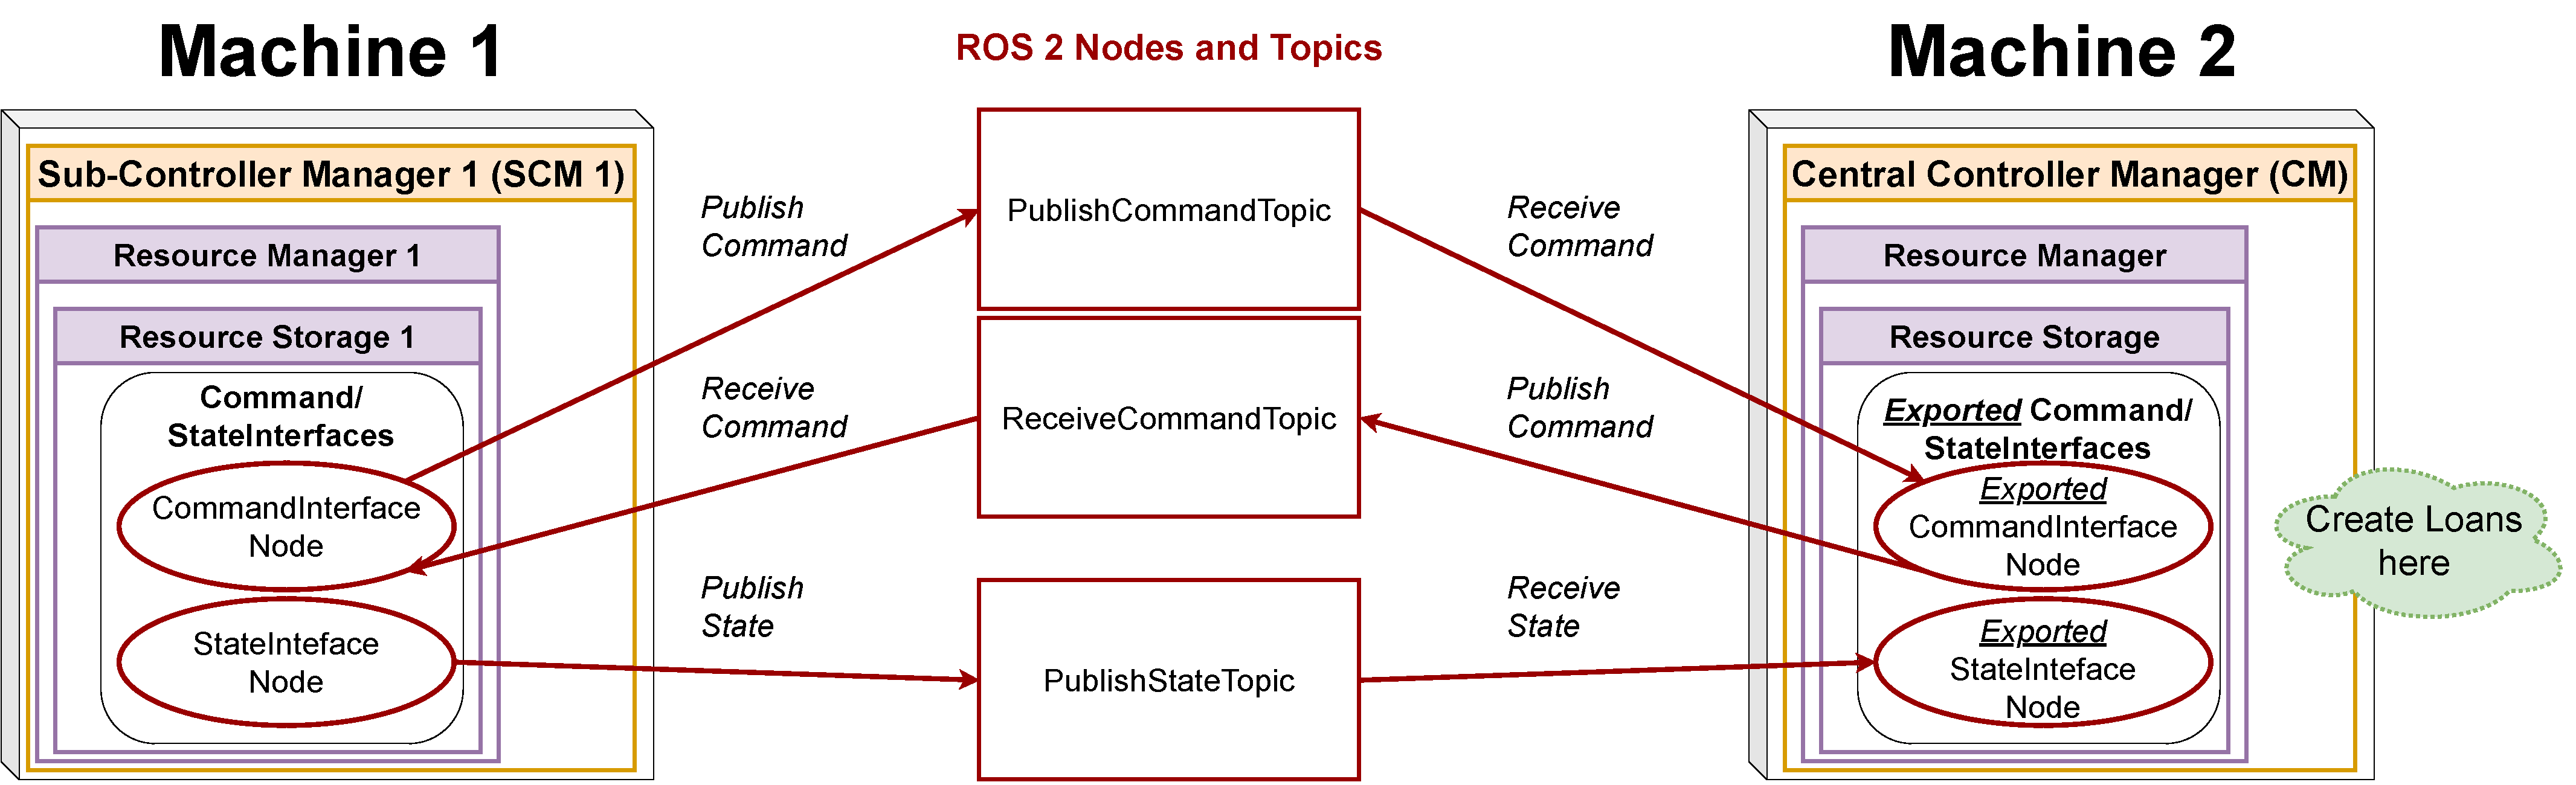
\includegraphics[width=1\textwidth]{Figures/C4/simple_concept.drawio.pdf}
	\caption{Schematic overview commands and states from one machine to another are transferred using topics and nodes from \gls{ros2}. The infrastructure provided by \gls{ros2} is thereby emphasized in red.}
	\label{c4_fig_simple_concept}
\end{figure}

\section{Integration in \gls{r2c}}
As described in section \ref{c3_sec_link_ctrl_hw} the current design of \gls{r2c} is built around a \gls{sm} architecture. As a result the control of multiple robots is only possible in two ways: 
\begin{enumerate}
    \item On one machine with a tight synchronization. 
    \item On multiple machines with no significant synchronization at all.
\end{enumerate}
This has been elaborated in \ref{c3_sec_controlling_multiple_robots} in more detail. The goal of this work is to test whether it is possible in the context of \gls{r2c} to run multiple controllers on multiple machines and still allow tight synchronization.\newline
As shown in the UML class diagram in graphic \ref{c3_fig_ros2_control_uml} the link between the hardware site and the controllers in the \gls{r2c} framework are the \texttt{CommandInterfaces} and the \texttt{StateInterfaces}. See section \ref{c3_sec_link_ctrl_hw} for a more detailed explanation of the conceptual background. \newline
The fundamental idea of the design is to split the system at this point and allow multiple controller managers to coexist. The controller managers are thereby divided into two groups. The first group consisting of exactly one central controller manager and a second group composed of possibly multiple sub controller managers.
\begin{figure}[htbp]
	\centering
	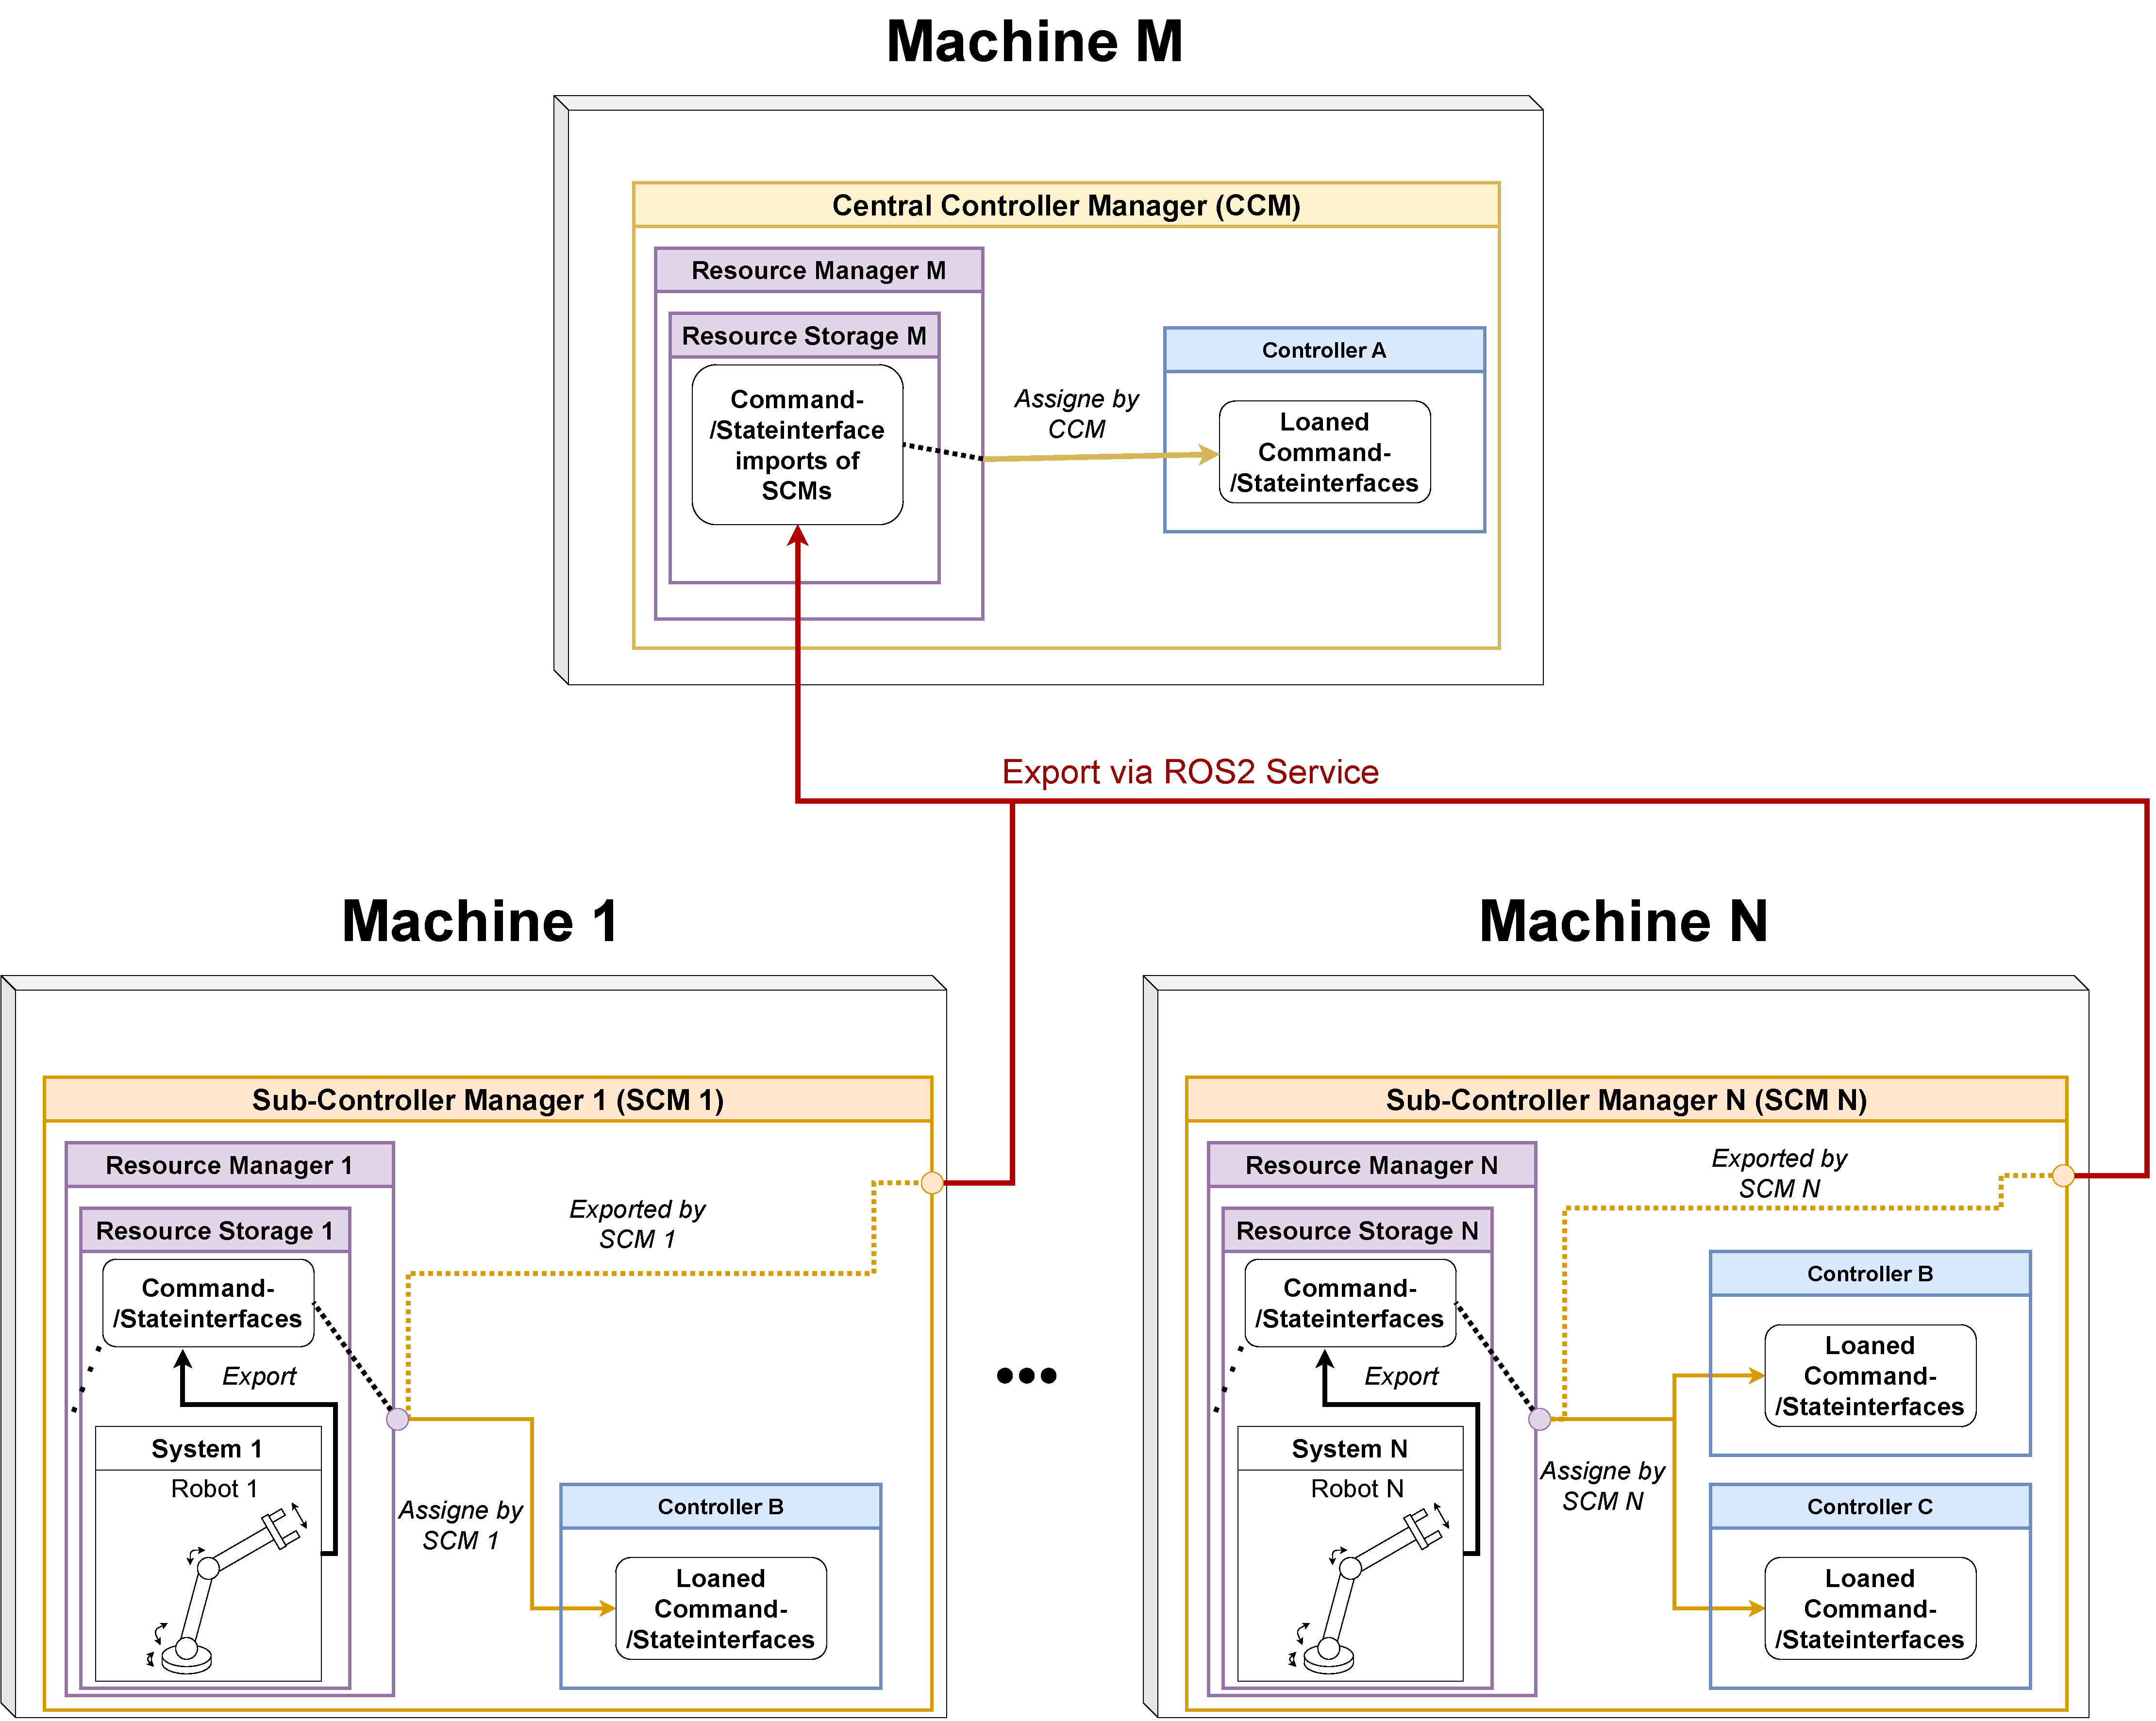
\includegraphics[width=1\textwidth]{Figures/C4/distributed_control.drawio.pdf}
	\caption{Schematic overview of the concept implemented. The figure shows, how a more complex system of multiple robots, controlled by multiple controllers on different machines, could be realized. }
	\label{c4_fig_concept_overview}
\end{figure}
\subsection{Central Controller Manager}
\begin{itemize}
    \item \textbf{Subcontroller manager:}
    \begin{itemize}
        \item register subcontroller manager $\implies$ export descriptions of Command-/SystemInterfaces
        \item create publisher for Command-/StateInterfaces
        \item wait for registration to successfully complete
        \item subscribe to commandpublisher received from central controller manager
    \end{itemize}
    \item \textbf{Central Controller manager:}
    \begin{itemize}
        \item create service for registration
        \item register subcontroller manger if receive call
        \item subscribe to publisher of Command-/StateInteface of subcontrolelr manager
        \item create special Command-/StateInterfaces for this
        \item create publisher for Commands
        \item proceed as normal
    \end{itemize}
\end{itemize}
\subsection{Controller Chaining}
\begin{itemize}
    \item \textbf{Subcontroller manager:}
    \begin{itemize}
        \item same as for simple case
        \item export additionally reference interfaces
    \end{itemize}
    \item \textbf{Central Controller manager:}
    \begin{itemize}
        \item same as simple case
        \item import reference interfaces
        \item create chained controller
        \item proceed as normal
    \end{itemize}
\end{itemize}

\begin{itemize}
    \item \textbf{Conceptual Design:}
    \begin{itemize}
        \item split at the handles
        \item have central- and subcontrollermanagers
        \item use topics to publish data
    \end{itemize}
    \item \textbf{Integration into \gls{r2c}}
    \item Separated drivers:
    \begin{itemize}
        \item registration
        \item creation of topics
    \end{itemize}
        \item Controller Chaining:
    \begin{itemize}
        \item registration
        \item creation of topics
        \item activation of chain
    \end{itemize}
\end{itemize}